\documentclass[a4paper, 12pt]{article}%тип документа



%отступы
\usepackage[left=1cm,right=1cm,top=1cm,bottom=2cm,bindingoffset=0cm]{geometry}

%%% Работа с русским языком
\usepackage{graphicx}
\usepackage{cmap}                           % поиск в PDF
\usepackage{mathtext} 			 	       % русские буквы в формулах
\usepackage[T2A]{fontenc}               % кодировка
\usepackage[utf8]{inputenc}              % кодировка исходного текста
\usepackage[english,russian]{babel} 
\usepackage{float}
\usepackage{caption}

\usepackage[export]{adjustbox} % локализация и переносы

\usepackage{subfig}% http://ctan.org/pkg/subfig
\usepackage{booktabs}

\usepackage{wrapfig}


%Матеша
\usepackage{amsmath,amsfonts,amssymb,amsthm,mathtools} % AMS
\usepackage{icomma} % "Умная" запятая

%\mathtoolsset{showonlyrefs=true} % Показывать номера только у тех формул, на которые есть \eqref{} в тексте.

%% Шрифты
\usepackage{euscript}	 % Шрифт Евклид
\usepackage{mathrsfs} % Красивый матшрифт

%% Свои команды
\DeclareMathOperator{\sgn}{\mathop{sgn}}

%% Перенос знаков в формулах (по Львовскому)
\newcommand*{\hm}[1]{#1\nobreak\discretionary{}
	{\hbox{$\mathsurround=0pt #1$}}{}}




\author{Гаврилин Илья Дмитриевич \\
	Б01-101}
\title{\textbf{Работа 2.5.1 \\ 
		Измерение коэффициента поверхностного натяжения жидкости}}

\begin{document}
	\maketitle
	\section{Аннотация}
		В работе определили зависимость коэффициента поверхностного натяжения воды от температуры $\sigma(T)$, с учетом известного коэффициента для спирта.Определили полную поверхностную энергию  и теплоту, необходимую для изотермического образования единицы  поверхности жидкости  при различной температуре. Оценили погрешности полученных величин.
	\section{Теоретические сведения}
		Наличие поверхностного слоя приводит к различию давлений по разные стороны от искривленной границы раздела двух сред.  Для сферического пузырька с воздухом  внутри жидкости избыточное давление даётся формулой Лапласа:
		\begin{equation}
			\Delta P = P_{in} - P_{out} = \dfrac{2 \sigma}{r} 
		\end{equation}
		где $\sigma$ - коэффициент поверхностного натяжения, $P_{in}$ и $P_{out}$ - давление внутри пузырька и снаружи, $r$ - радиус кривизны поверхности раздела двух фаз. Эта формула лежит в основе предлагаемого метода определения коэффициента поверхностного натяжения жидкости. Измеряется давление $\Delta P$, необходимое для выталкивания в жидкость пузырька воздуха.
		\begin{figure}[H]
			\centering
			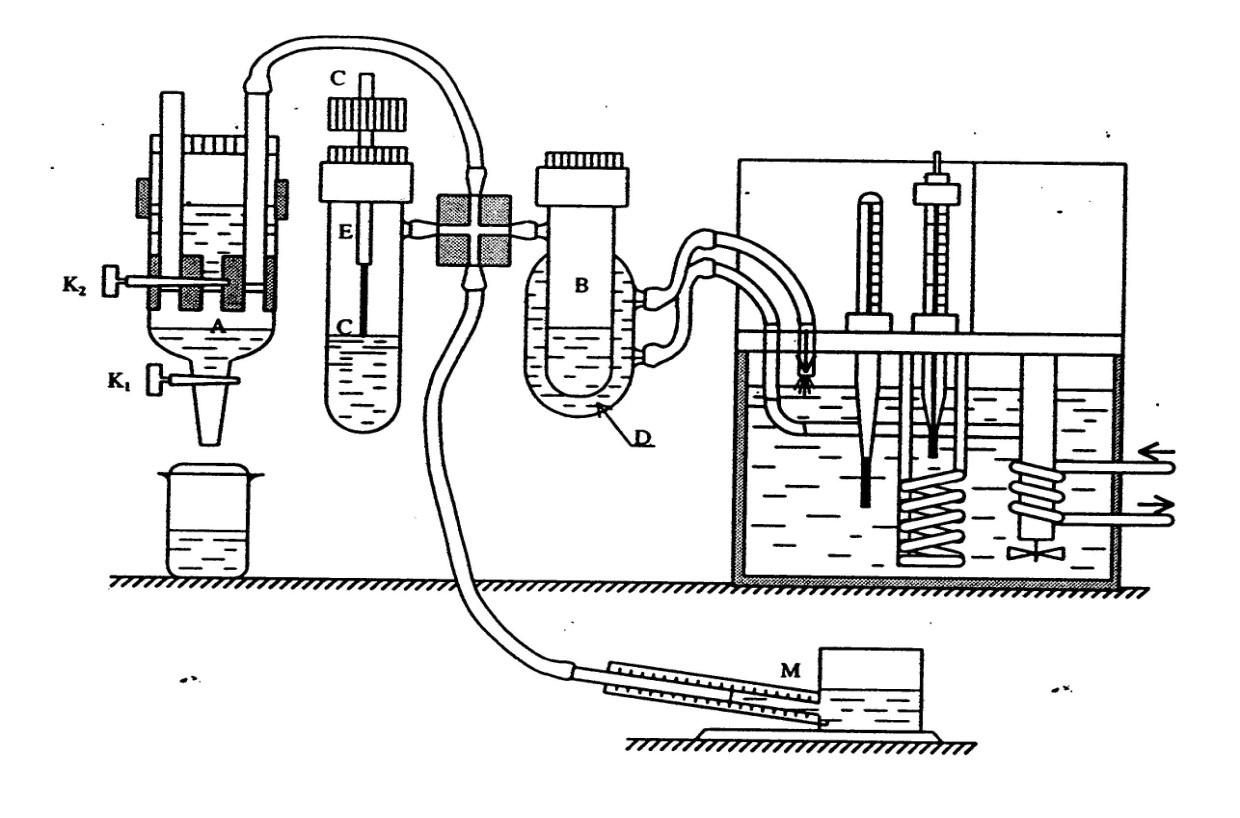
\includegraphics[width = 0.6\textwidth, angle=0.8]{251_1.jpg}
			\caption{Схема экспериментальной установки}
		\end{figure}
	\section{Ход работы}
		Проверим установку на герметичность путем наблюдения установления давления на манометре при перекрытии крана с каплями. Выставим частоту падения капель не чаще одной в 5 секунд.\\
		\subsection{Замер диаметра иглы}
		Замерим диаметр иглы двумя способами: напрямую с помощью микроскопа и при помощи известного значения коэффициента поверхностного натяжения для спирта.
		\begin{figure}[H]
			\begin{center}
				\begin{minipage}[h]{0.48\linewidth}
					\centering
					\begin{tabular}{|c|c|c|c|c|c|}
						\hline
						N замера        & 1     & 2     & 3     & 4     & 5     \\ \hline
						P, усл. ед.\footnote{Здесь и далее усл. ед. означают прямые показания на манометре при том что $1~ усл.~ ед. \approx 1.96 ~Па $}     & 44    & 45    & 43    & 46    & 45    \\ \hline
						$R_{иглы}$, мм & 0.527 & 0.516 & 0.540 & 0.504 & 0.516 \\ \hline
					\end{tabular}
					\captionof{table}{Замер радиуса с помощью известного коэффициента поверхностного натяжения спирта.}
					\end{minipage}
				\hfill
				\begin{minipage}[h]{0.48\linewidth}
					\centering 
					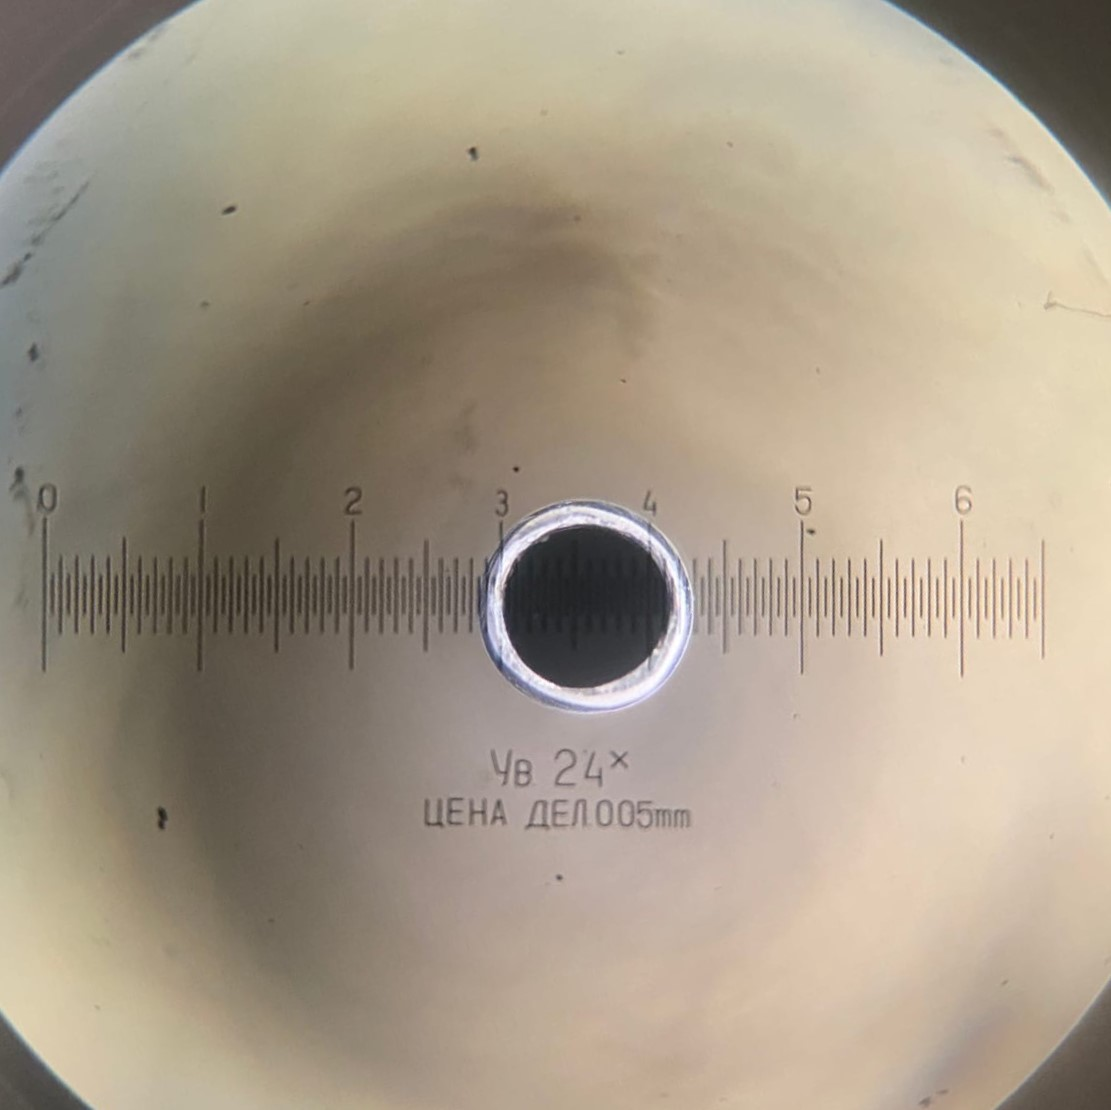
\includegraphics[width=0.7\linewidth]{needle.jpg} 
					\caption{Измерение диаметра иглы микроскопом} 
				\end{minipage}
			\end{center}
		\end{figure}
		Для измерения с помощью спирта по формуле (1) получаем:\\ $ \overline{R}  = 0.520~мм,~\overline{D}  = 1.04~мм,~\delta_{случ}$\footnote{Символ $\sigma$ задействован в качестве коэффициента поверхностного натяжения, поэтому погрешность обозначаем $\delta$}$ (R) = 0.012~мм $. Однако, мы еще не учли приборную погрешность манометра, которая оказывается достаточно большой, и тогда полная погрешность равна:\newline $\delta_{\sum}(D)=0.07~ мм$.\\
		Для измерения диаметра с помощью микроскопа получаем (проведем несколько замеров немного двигая иглу, чтобы убедиться в правильности замера): $\overline{D} = 1.15~ мм, \delta(D)=0.05~мм$.\\
	\textbf{Итого, выбирая метод с наименьшей погрешностью: $D_{иглы}=1.15\pm 0.05 ~мм$.}
	\subsection{Измерение добавочного давления при погружении иглы}
	Замерим избыточное давление, образуемое при погружении иглы на глубину $\Delta h$: с помощью сравнения $\Delta P$ погруженной и лишь касающейся воды иглы и с помощью прямого измерения $\Delta h$ линейкой.\newline
	С помощью линейки: $\Delta h = 1.25\pm 0.05 ~см, \Delta P = \rho g \Delta h = 122.4\pm4.8~ Па$.\\
	Напрямую измеряя разность давлений на поверхности и на глубине: \newline
	$\Delta P_{1} = 243.2~Па, \Delta P_{2} = 366.8 ~Па, \Delta P = 123.6\pm 0.8~Па$.\newline
	\textbf{Итого, выбирая метод с наименьшей погрешностью: $\Delta P = 123.6\pm 0.8~Па$.}
	\subsection{Проведение основных измерений, получение зависимости $\sigma(T)$}
	Зафиксируем иглу при максимальном погружении, для которого был получен параметр $\Delta P_{изб}$, будем менять температуру с интервалом 5 градусов цельсия и фиксировать значения для построения графика $\sigma(T)$	\begin{table}[H]
		\centering
		\begin{tabular}{|c|c|c|c|}
			\hline
			T, K & $\Delta P$, усл. ед. & $\Delta P$, Па & $\sigma~ *10^{-3} ~\frac{H}{м}$ \\ \hline
			293.2       & 187              & 243.20       & 69.9  \\ \hline
			298.2       & 181              & 231.44       & 66.5  \\ \hline
			303.1       & 180              & 229.48       & 66.0  \\ \hline
			308         & 179              & 227.51       & 65.4  \\ \hline
			313         & 179              & 227.51       & 65.4  \\ \hline
			318         & 178              & 225.55       & 64.8  \\ \hline
			323         & 177              & 223.59       & 64.3  \\ \hline
			328         & 175              & 219.67       & 63.2  \\ \hline
			333         & 174              & 217.71       & 62.6  \\ \hline
		\end{tabular}
		\caption{Зависимость коэффициента поверхностного натяжения воды от температуры}
	\end{table}
	При подсчете $\Delta P$ учитывается избыточное давление $\Delta P_{изб}$, чтобы зразу получить давление, нужное для формулы (1). Оценим погрешность определения $\sigma$: для каждого значения $\sigma$ получили схожие погрешности (ввиду падения относительной погрешности определения давления). $\delta(\sigma) \approx 0.4 \frac{Н}{м}$ \\
	Построим график $\sigma(T)$ и по угловому коэффициенту наклона найдем $\frac{d\sigma}{dT}$. Точка, соответствующая температуре 293.2 К, плохо ложится на прямую аппроксимирующую точки, поэтому при аппроксимации она не учитывалась.
	\begin{figure}[H]
		\centering
		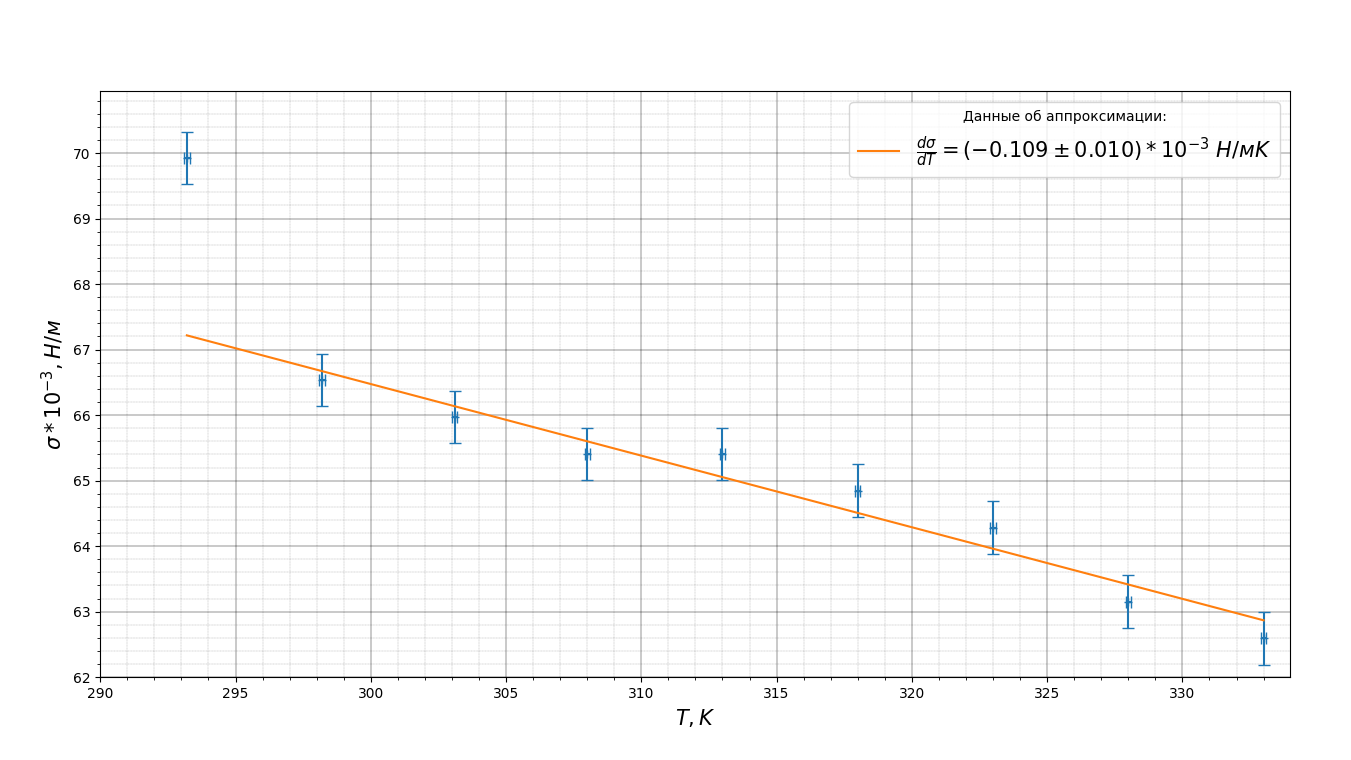
\includegraphics[width=0.8\linewidth]{graph_sigma}
		\caption{Зависимость коэффициента поверхностного натяжения от температуры}
		\label{fig:graphsigma}
	\end{figure}
	Из аппроксимации получили $\frac{d\sigma}{dT} = -(0.109\pm 0.010) * 10^{-3}~\frac{Н}{мК}$. Из полученных данных построим: \\1)график теплоты образования единицы поверхности жидкости  от температуры $q = -T\frac{d\sigma}{dT}$(рис. 4); \\2)поверхностной энергии U единицы площади F от температуры $\frac{U}{F} = (\sigma - T\frac{d\sigma}{dT})$(рис. 5).\\
	\begin{figure}[H]
		\begin{center}
			\begin{minipage}[h]{0.48\linewidth}
				\centering 
				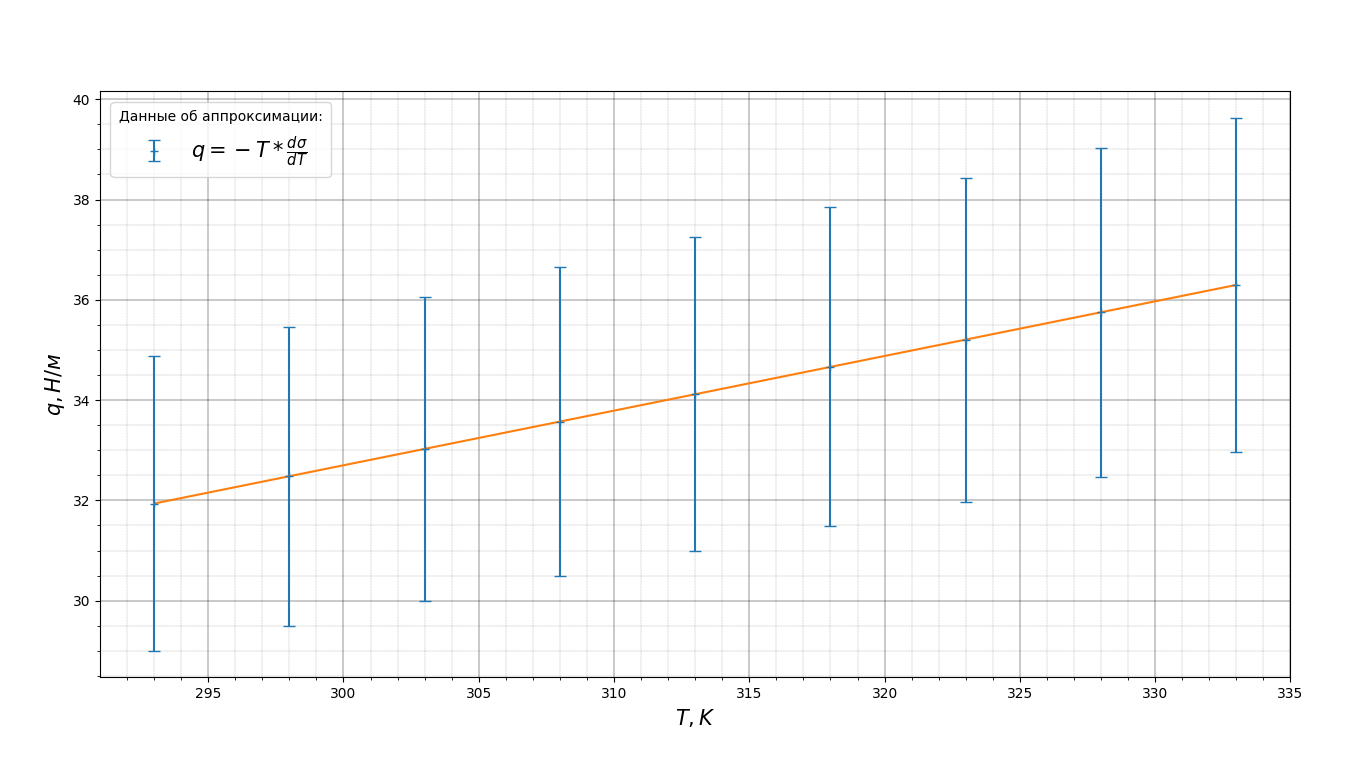
\includegraphics[width=1\linewidth]{graph_q} 
				\caption{Теплота образования единицы поверхности от температуры}
			\end{minipage}
			\hfill
			\begin{minipage}[h]{0.48\linewidth}
				\centering 
				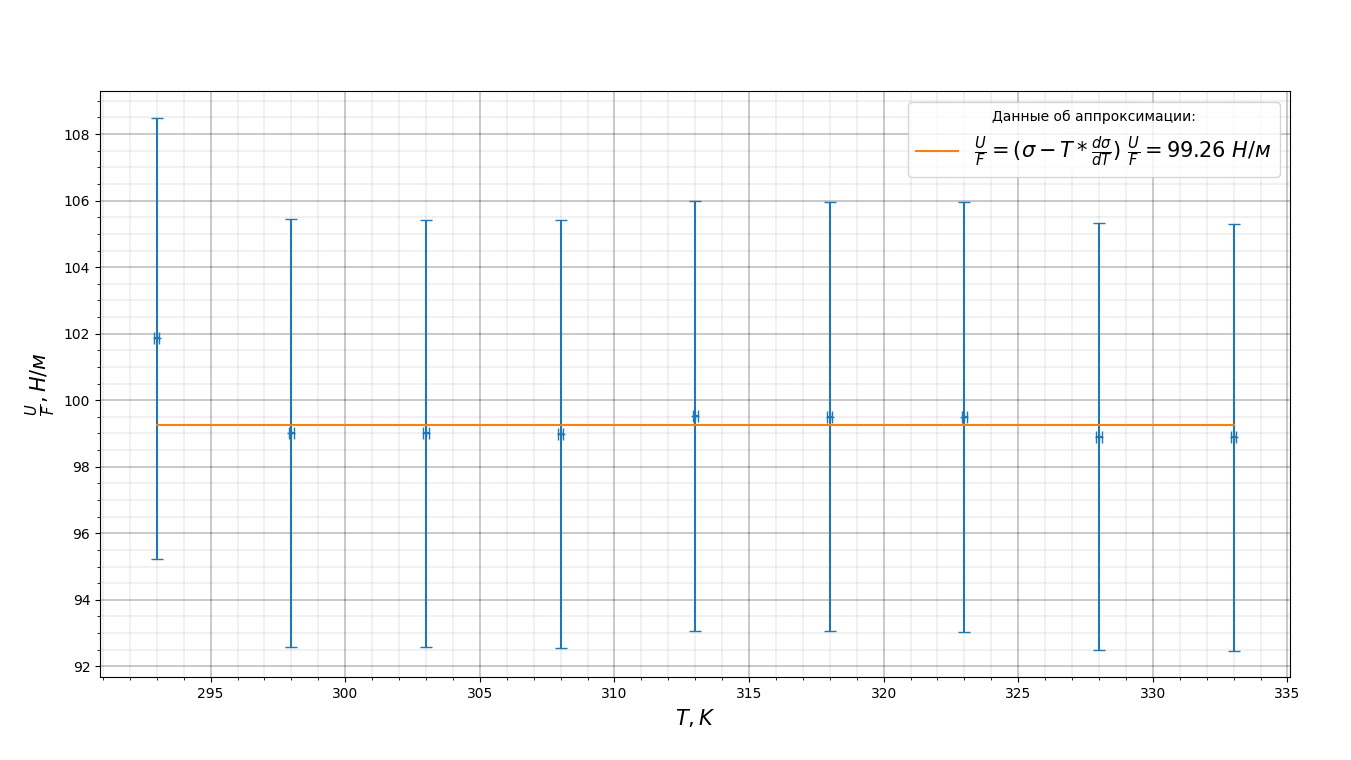
\includegraphics[width=1\linewidth]{graph_u} 
				\caption{Поверхностная энергия единицы площади от температуры} 
			\end{minipage}
		\end{center}
	\end{figure}
	\section{Вывод}
	В работе замерили значения коэффициента поверхностного натяжения воды от температуры, изучили зависимость $\sigma(Т)$, она оказалась линейной, с угловым коэффициентом:  $\frac{d\sigma}{dT} = -(0.109\pm 0.010) * 10^{-3}~\frac{Н}{мК}$.\\
	Сравнили полученные значения поверхностного натяжения с табличными, отклонение не превысило 10\%.\\
	\begin{table}[H]
		\centering
		\begin{tabular}{|c|c|c|c|c|c|}
			\hline
			T, K    & 293.2 & 303.1 & 313   & 323   & 333   \\ \hline
			$\sigma_{эксп}~ *10^{-3} ~\frac{H}{м}$    & 69.92 & 65.97 & 65.41 & 64.28 & 62.59 \\ \hline
			$\sigma_{табл}~ *10^{-3} ~\frac{H}{м}$   & 72.75 & 71.18 & 69.56 & 67.91 & 66.18 \\ \hline
			$\epsilon, ~\%$ & 3.9   & 7.3   & 6.0   & 5.3   & 5.4   \\ \hline
		\end{tabular}
		\caption{Отклонение значений коэффициента поверхностного натяжения воды от табличных.}
	\end{table}
	Также, построили графики теплоты образования единицы поверхности и поверхностной энергии единицы площади. Выяснили, что рост теплоты образования единицы поверхности схож с линейным, однако, о какой-либо зависимости поверхностной энергии от температуры говорить сложно.
\end{document}
